\documentclass{article}
\usepackage{tikz,pgfplots}
\usetikzlibrary{positioning}

\begin{document}

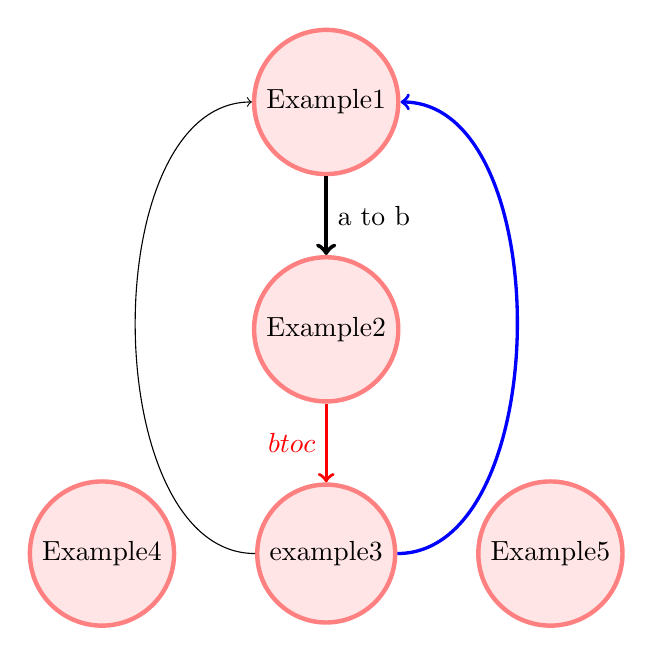
\begin{tikzpicture}[rs/.style={circle, draw=red!50, fill=red!10, ultra thick, minimum size=10mm}
	]
	
	\node[rs] (a) [draw] {Example1};
	\node[rs] (b)    [below=of a]   {Example2};
\node[rs] (c) [below=of b] {example3};
	
	\node [rs] (d) [left=of c] {Example4};
	\node [rs] (e) [right=of c] {Example5};
	%\node[rs] (f) [above=of a] {Example6};
	
	
	\draw [->, ultra thick] (a.south) to node [right]{a to b} (b.north);
	\draw [->,very thick,red] (b.south) to node[left] {$ b to c$} (c.north);
	
	\draw [->, very thick,blue] (c.east) .. controls + (right:20mm) and + (right:20mm) ..
	(a.east)
	;
	\draw [->, thin] (c.west) .. controls + (left:20mm) and + (left:20mm) .. (a.west);
	
	
\end{tikzpicture}
\end{document}